% Autor: Jose Ricardo Bustos Molina
%        Universidad del Tolima
%        jrbustosm@ut.edu.co
%
\section{Antecedentes}

Para investigar el estado académico actual acerca de la influencia de la gamificación y los juegos de rol 
sobre la motivación de los estudiantes, se realizó una revisión sistemática de literatura utilizando las bases 
de datos Science direct, Springer link, Scopus, Oxford academic, Google scholar, EBSCO y el gestor de la 
biblioteca de la Universidad del Tolima y demás universidades con programas de maestría en el área de 
educación, como se muestra en el modelo de la Figura \ref{img:busqueda}. Para implementar esta búsqueda se 
usó como fuente inicial la cadena de búsqueda:

\begin{center}\ttfamily\sbox{0}{a}    % Poner tipo de fuente
\begin{minipage}{64\wd0}              % página de 64 caracteres
\begin{verbatim}
(gamif* OR rol* game) AND (motivation) OR (gamif* AND rol* game)
      LIMIT(10 year), AREA(social sciences AND psychology)
\end{verbatim}
\end{minipage}
\end{center}

\begin{figure}[ht]
\caption{Modelo búsqueda sistemática bibliografía}
\label{img:busqueda}
\centering
\begin{tikzpicture}[
		every node/.append style={draw=gray!80,align=center,minimum width=90pt,very thin}
  	]
	\node (I) at (-3.5,-1.5) {
		\textbf{\small Inicio}
	};
	\node (CB) at (-3.5,0.5) {
		\textbf{\small Cadena de Búsqueda}\\{\scriptsize (gamif* OR rol* game) AND}\\
		{\scriptsize (motivation) OR (gamif* AND rol* game)}\\
		{\scriptsize LIMIT(10 year),}\\
		{\scriptsize AREA(social sciences AND psychology)}
	};
	\node (BD) at (-3.5,4) {
		\textbf{\small Base de Datos}\\{\scriptsize Science direct, Springer link, Scopus,}\\{\scriptsize Oxford Academic, google scholar, EBSCO, UT}
	};
	\node (WC) at (2.7,0.5) {
		\textbf{\small Nubes de Palabras}\\ \includegraphics[width=.3\textwidth]{img/keywords_count_full}
	};
	\node (E) at (2.7,4) {
		\textbf{\small Descarga Articulo/Metadatos}\\{\scriptsize Título, Autores, Resumen, Año,}\\{\scriptsize Palabras Clave, Tipo, Publicación}
	};
	\node (R) at (5.7,5.5) {
		\textbf{\small Artículos recomendados (IA)}
	};
	\node (C) at (8,4) {
		\textbf{\small Clasificación (Jabref)}\\{\scriptsize Review, Gamificación, Narración,}\\{\scriptsize RPG, Motivación, Misceláneo}
	};
	\node (A) at (8,2.3) {
		\textbf{\small Anotación}
	};
	\node (An) at (8,0) {
		\textbf{\small Análisis}\\ \includegraphics[width=.2\textwidth]{img/teoriasYmodelos.sort}
	};
	\draw[-triangle 90] (I) edge (CB);
	\draw[-triangle 90] (CB) edge (BD);
	\draw[-triangle 90] (BD) edge (E);
	\draw[-triangle 90] (E) edge (WC);
	\draw[-triangle 90] (WC) edge (CB);
	\draw[-triangle 90] (E) edge (C);
	\draw[-triangle 90] (C) edge (A);
	\draw[-triangle 90] (A) edge (An);
	\draw[-triangle 90,dashed] (E) edge (R);
	\draw[-triangle 90,dashed] (R) edge (C);
\end{tikzpicture}
{\footnotesize Fuente: de elaboración propia.}
\end{figure}

En la búsqueda sistemática se limitó a metadatos, que incluían títulos, resúmenes y palabras clave. Se realizó 
el análisis de nuevos términos de búsqueda usando nubes de palabras generadas a partir de los resúmenes y las 
palabras claves de los artículos seleccionados (ver Figura \ref{img:nube}), para modificar las respectivas 
cadenas de búsqueda y volver a repetir el proceso usando nuevos términos. 

\begin{figure}[ht]
  \caption{Nubes de palabras generadas}
  \label{img:nube}
  \centering
  \subfloat[A partir de los títulos y resúmenes]{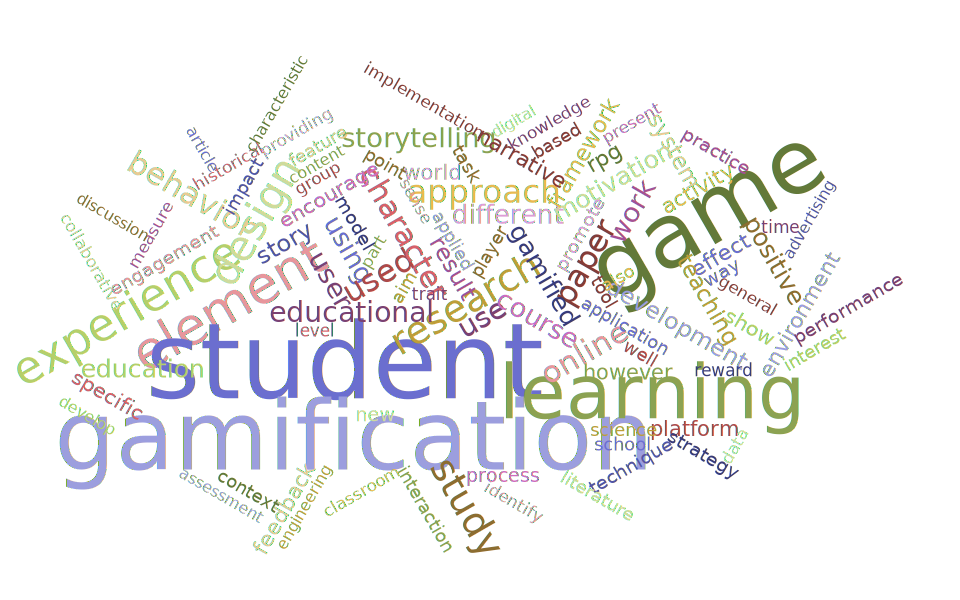
\includegraphics[width=0.45\textwidth]{abstracts_count_lemmatize}\label{img:nubef1}}
  \hfill
  \subfloat[A partir de las palabras claves]{\includegraphics[width=0.45\textwidth]{keywords_count_full}\label{img:nubef2}}
  \\
  {\footnotesize Fuente: de elaboración propia.}
\end{figure}

Si bien existe una cantidad sustancial de investigación en gamificación, solo una minoría de estas 
publicaciones utiliza juegos de rol o la narración de historias como un complemento. En total, se encontraron
76 publicaciones que cumplían los parámetros deseados, 29 del orden regional y 47 del orden internacional, 
donde 54 documentos tratan sobre gamificación, 13 tratan de la narración de historias, 14 tratan el tema de 
juegos de rol y 7 sobre teorías de motivación, de estos trabajos, hay 10 que combinan las estrategias de 
juegos de rol con gamificación y 9 que mezclan la estrategia de narración de historias con la gamificación. 
Esto se puede ver resumido en la Figura \ref{img:catbib}.

En cuanto al tipo de publicación encontrada son 30 artículos, 26 tesis de maestría, 11 libros, 6 artículos de 
conferencias, y 3 capítulos de libro. Además, 68 de estas publicaciones son de los últimos 10 años y 8 de años 
anteriores.

Por otra parte, es importante resaltar que de los 54 estudios sobre gamificación, 52 estudios arrojaron 
resultados motivacionales o relacionados con el desempeño o la motivación positivos o ligeramente positivos, 
mientras que dos estudios encontraron resultados mixtos \cite{DING20191, PRESTOPNIK2015492}.

\begin{figure}[ht]
\caption{Resumen categorías de bibliografía}
\label{img:catbib}
\centering
\begin{tikzpicture}[pattern color=lightgray, pattern=north east lines]
	\scope
	\clip (-3,0) circle (2);
	\fill (0,0) circle (2);
	\endscope
	\scope
	\clip (3,0) circle (2);
	\fill (0,0) circle (2);
	\endscope
	\draw (-3,0) circle (2) (-3,2.4)  node {Juegos de Rol} (-3,0)  node {\LARGE 4};
	\draw (-1.5,0)  node {\Large 10};
	\draw (3,0) circle (2) (3,2.4)  node {Narración} (3,0)  node {\LARGE 4};
	\draw (1.5,0)  node {\Large 9};
	\draw (0,0) circle (2) (0,2.4)  node {Gamificación} (0,0)  node {\LARGE 35};
	\draw (7,0) circle (1.5) (7,1.9)  node {Otras} (7,0)  node {\LARGE 14};
	\draw (-6,-2.5) rectangle (9,3);
	\draw (7,3.4) node {H=76 publicaciones};
\end{tikzpicture}
\\
{\footnotesize Fuente: de elaboración propia.}
\end{figure}

\pagebreak

Adicional a esto, se usaron los textos completos para realizar un conteo de las teorías o modelos 
(psicológicos, pedagógicos o de aprendizaje) mencionadas en los estudios, mostrando predominancia en cuanto a 
dos teorías en particular: teoría de la autodeterminanción y teoría de reforzamiento conductual, 
como se puede ver en la Figura \ref{img:nubeteorias}.

\begin{figure}[H]
  \caption{Nubes de palabras generadas para teorías y modelos}
  \label{img:nubeteorias}
  \centering
  \includegraphics[width=0.8\textwidth]{teoriasYmodelos.sort}
  \\
  {\footnotesize Fuente: de elaboración propia.}
\end{figure}

\subsection{Antecedentes regionales del uso de estrategias de gamificación o juegos de rol en educación}

En el contexto del departamento del Tolima y con el objetivo de establecer antecedentes sobre gamificación, se 
presentan adicionalmente investigaciones en contexto local que usan la lúdica como eje fundamental del 
aprendizaje, en cuanto al contexto nacional se hace especial énfasis en trabajos de maestría que desarrollen 
la categoría de gamificación y el uso de juegos de Rol, mas no el desarrollo de juegos serios. Por lo tanto,
se implemento una búsqueda sistemática para el descubrimiento de tesis a nivel de maestría o doctorado, en los
diferentes motores de búsqueda implementados en los portales de bibliotecas de cada Universidad, obteniendo un 
total de 25 tesis todas ellas a nivel de maestría, de 14 instituciones diferentes las cuales se pueden ver 
resumidas en la tabla \ref{tab:resumenlocal}.

\begin{table}[!htb]
\caption{Resumen tesis de maestría gamificación/juego de roles a nivel nacional}
\label{tab:resumenlocal}
\begin{center}
\footnotesize
\begin{tabular}{ p{50mm} p{50mm} p{15mm} c}
\toprule
	\textbf{Universidad} & \textbf{Programa(s)} & \textbf{Ciudad} & \textbf{Cantidad}\\ 
\midrule
	Pontificia Universidad Javeriana & Maestría en Ingeniería Electrónica & Bogotá & 1\\
	Universidad Cooperativa de Colombia & Maestría en Educación & Bogotá & 1\\
	Universidad de Antioquia & Maestría en Educación & Medellín & 1\\
	Universidad de la Costa & Maestría en Educación & Barranquilla & 1\\
	Universidad de los Andes & Maestría en Educación & Bogotá & 1\\
	Universidad de Santander UDES & Maestría en Tecnologías Digitales Aplicadas a la Educación & Bogotá & 
	1\\ 
	Universidad del Tolima & Maestría en Educación & Ibagué & 3\\
	Universidad Icesi & Maestría en Educación & Santiago de Cali & 2\\
	Universidad Nacional de Colombia sede Bogotá & Maestría en Ingeniería – Ingeniería de Sistemas y 
		Computación / Maestría Enseñanza de las Ciencias Exactas y Naturales & Bogotá & 2\\
	Universidad Nacional de Colombia sede Medellín & Maestría Enseñanza de las Ciencias Exactas y 
		Naturales & Medellín & 4\\
	Universidad Pedagógica Nacional & Maestría Tecnologías de la Información Aplicadas a la Educación & 
		Bogotá & 1\\
	Universidad Pontificia Bolivariana & Maestría en Educación & Medellín & 1\\
	Universidad Tecnológica de Bolívar & Maestría en Educación/Maestría en Gestión De La Innovación & 
		Cartagena &  4\\
	UPTC, Universidad Pedagógica y Tecnológica de Colombia & Maestría en TIC Aplicadas a las Ciencias de 
		la Educación & Duitama & 1\\
\bottomrule
	\multicolumn{4}{l}{\footnotesize Fuente: de elaboración propia.}\\
\end{tabular}
\end{center}
\end{table}

%Con un enfoque más amplio, \citeA{villamil2016} en su proyecto ``Los videojuegos, nuevas narrativas del siglo 
%XXI'', que contextualización los conceptos básicos del juego con el fin de alcanzar un mejor el desarrollo 
%cognitivo y emocional, usando diferentes análisis de narración a diferentes videojuegos estudiados, 
%complementando con un estudio de los procesos creativos que involucran la realización de argumentos y guiones 
%en videojuegos.

En el presente estudio, no se pudo evidenciar localmente trabajos sobre gamificación a nivel de maestría o 
doctorado, sin embargo, si se encuentran tres trabajos relacionados al tema sin que este sea su eje principal,
por ejemplo, \citeA{barragan2015}, en su trabajo ``Square Game como apoyo del proceso de evaluación de la 
geometría en el segundo grado de básica primaria de la región Alto Magdalena - Colombia'', que plantea el 
desarrollo de un juego serio basado en Tangram para simplificar procesos cognitivos en la enseñanza de la 
geometría, consiguiendo un aprendizaje significativo en el aprendizaje de figuras geométricas básicas en los 
estudiantes.

Adicional a esto, \citeA{lobo2015} en su proyecto ``Estrategia metodológica basada en la actividad lúdica para 
el desarrollo del pensamiento variacional en estudiantes de 8º grado que cursan la asignatura matemática en la 
institución educativa rural San Joaquín del municipio de Santa María-Huila'' quienes proponen una estrategia 
metodológica basada en la lúdica para potenciar el desarrollo del pensamiento matemático (propiedades, 
lenguaje algebraico, operaciones y resolución de problemas) en los estudiantes y un estudio cualitativo de su 
implementación.

Finalmente, \citeA{garcia2014}, en su estudio ``Uso pedagógico del celular en el aula'', cuyo propósito fue 
estimar la tenencia de teléfonos celulares por parte de estudiantes y profesores, mostrándonos un escenario 
idóneo para propiciar eventos de enseñanza-aprendizaje usando los móviles como medio de mediación.

En cuanto al contexto nacional, son varios los que hacen uso extensivo de la gamificación como estrategia para
el aprendizaje, por ejemplo \citeA{Mera-Paz_2016} realiza una reflexión sobre la gamificación como estrategia 
para el fortalecimiento del pensamiento algorítmico en el programa ingeniería de sistemas de la Universidad 
Cooperativa de Colombia sede Popayán, y \citeA{MORENO2015} quienes crean y evalúa una estrategia didáctica 
gamificada implementada en un ambiente virtual para los cursos de pre-cálculo de la Universidad Nacional de 
Colombia, mostrando un incremento en el desempeño académico y en el porcentaje de aprobación, al tiempo que
una disminución en el abandono estudiantil.

De acuerdo con la búsqueda realizada de tesis a nivel de maestría en Colombia, los diferentes estudios se 
pueden clasificar en tres grandes grupos: orientados a la educación escolar, a la participación ciudadana y 
bajo un contexto empresarial. Sin embargo, el número de trabajos de estos dos últimos grupos es mas bajo (4 
trabajos en total), respecto al uso de gamificación o juegos de rol en el ambiente educativo, que es donde se 
encuentra el grueso de los esfuerzos de investigación en los diferentes programas de maestría (18 en total), 
incluyendo dos trabajos que usan los juegos de rol en conjunto con la gamificación como estrategia de 
enseñanza.

Anudando a lo anterior, el uso de estrategias gamificadas o juegos de rol en la educación, se pudo evidenciar
su uso en la enseñanza del área de ciencias naturales (9 trabajos), ciencias humanas (3 trabajos), tecnología 
(1 trabajo), idioma extranjero (2 trabajos), matemáticas (2 trabajos) y un estudio genérico. A continuación, a 
manera de resumen, se muestra en la tabla \ref{tab:bioanotada} la bibliografía anotada anteriormente descrita 
y clasificada.

\begin{center}
\footnotesize
\begin{longtable}{ p{25mm} p{50mm} p{75mm} }
	\caption{Bibliografía anotada de tesis de maestría en Colombia, tema: Gamificación y Juegos de Rol}
	\label{tab:bioanotada} \\

	\toprule
	\textbf{Autores} & \textbf{Título} & \textbf{Anotación}\\
	\midrule
	\endfirsthead
	
	\toprule
	\textbf{Autores} & \textbf{Título} & \textbf{Anotación}\\
	\midrule
	\endhead

	\midrule
	\multicolumn{3}{r}{{Continúa en la siguiente página\dots}} \\
	\bottomrule
	\endfoot

	\bottomrule
	\multicolumn{3}{l}{\footnotesize Fuente: de elaboración propia.}\\
	\endlastfoot

\citeA{Albornoz2021} & Estrategia Didáctica Basada en la Gamificación para el Fortalecimiento de las 
Habilidades Investigativas en Estudiantes de Grado Sexto (\textbf{Universidad de Santander UDES}) & Se 
desarrolla un trabajo que mediante un diseño de un curso virtual que usa gamificación fortalezca las 
habilidades investigativas en estudiantes de grado sexto, estudio con enfoque \uline{cualitativo}, encontrando 
una mejora a partir de la implementación de la estrategia didáctica gamificada respecto al grupo de control.\\
\citeA{Arias2021} & La gamificación como estrategia que contribuye al desarrollo del uso comprensivo del 
conocimiento científico mediante la enseñanza del sistema digestivo humano (\textbf{Universidad Nacional de Colombia}) 
& Estrategia gamificada implementada en estudiantes de grado quinto para el aprendizaje del sistema digestivo, 
usando un enfoque \uline{cualitativo} con una metodología de \uline{investigación-acción}, concluyendo que 
esta contribuye de una forma positiva a la comprensión por parte de los estudiantes, pudiendo evidenciar 
exitosamente el interés en los estudiantes\\
\citeA{Arias2012} & Uso de un juego de rol como herramienta de motivación en la enseñanza de la química 
(\textbf{Universidad Nacional de Colombia}) & Muestra el uso de un juego de rol como estrategia para aumentar 
la motivación en la enseñanza de la química orgánica en un curso de educación superior, usando elementos de 
\uline{aprendizaje basado en problemas y colaborativo}, encontrando resultados positivos en cuanto a 
motivación, participación y aprendizaje, adicionalmente mejorando la relación docente-estudiante.\\
\citeA{betancur2018} & La literatura infantil y juvenil, desde la gamificación: un escenario posible para la 
formación literaria en la básica primaria (\textbf{Universidad de Antioquia}) & Investigación que busca 
fortalecer la formación literaria en estudiantes del grado tercero, usando técnicas gamificadas y un enfoque 
\uline{cualitativo} en la investigación, encontrando que la implementación de este tipo de estrategias 
favorece el desarrollo de diversas competencias lingüísticas y comunicativas en los estudiantes, mejorando
los hábitos lectores, y un incrementó en el interés frente a la literatura y el proceso lector.\\
\citeA{Buitrago2021} & Estrategia de gamificación para la enseñanza y evaluación de la estructura atómica en 
la educación básica en el contexto rural (\textbf{Universidad Nacional de Colombia}) & Plantea una estrategia 
gamificada usando el \uline{aprendizaje basado en problemas}, para la enseñanza de la estructura de los átomos 
en estudiantes de grado sexto, usando un enfoque \uline{cualitativo} y bajo el paradigma critico social 
(modelo de investigación acción educativa), encontrando una mejoría respecto a la actitud por parte de los 
estudiantes, respecto a los tiempos y compromisos en las clases síncronas mediadas por TICs.\\
\citeA{camacho2020} & Estrategia didáctica de gamificación y juego de rol para la promoción de la convivencia 
y la paz en estudiantes de tercero de primaria (\textbf{Universidad Icesi}) & Desarrolla un juego de rol 
gamificado para educar habilidades en la convivencia escolar y la paz, en estudiantes de tercero de primaria. 
Mediante el uso de un enfoque \uline{cualitativo}, se encuentra que la estrategia aportó en el desarrollo 
afectivo emocional de los estudiantes, logrando entretenerlos y estimularlos, fortaleciendo la capacidad de 
diálogo, y la capacidad de generar acuerdos comunes en la resolución de conflictos.\\
\citeA{cano2019} & Un estudio comparado sobre gamificación en dos contextos educativos del área metropolitana 
del valle de aburrá (\textbf{Universidad Pontificia Bolivariana}) & Este trabajo de investigación propone la 
aplicación de una estrategia gamificada en dos instituciones educativas diferentes, el estudio presenta un
enfoque \uline{cualitativo} y con un \uline{diseño cuasiexperimental}, encontrando un impacto positivo en el 
rendimiento académico de los estudiantes, permitiendo encontrar un aumento en los niveles de motivación y
compromiso.\\
\citeA{Cuervo2021} & Evaluación del efecto de la gamificación asistida por computador en la motivación de los 
estudiantes de programación de computadores (\textbf{Universidad Nacional de Colombia}) & Esta investigación 
tiene como propósito dimensionar el efecto que la gamificación en el aprendizaje de programación de 
computadores, en estudiantes de nivel universitario. Para tal fin, se emplea un \uline{enfoque mixto} y a 
través de un estudio \uline{cuasi-experimental}, encontrando un incremento significativo en los niveles 
relacionados con la valoración de tareas, atribuyendo un mayor grado de importancia, utilidad, gusto o 
interés por su realización.\\
\citeA{delahoz2015} & Gamificación para la gestión de la innovación en las organizaciones : caso empresa del 
sector químico de la ciudad de Barranquilla (\textbf{Universidad Tecnológica de Bolívar}) & Se desarrolla un 
proyecto que mediante el \uline{análisis de casos} con un enfoque \uline{cualitativo}, potencia la gestión de 
la innovación en las organizaciones privadas, usando el método de \uline{triangulación de datos} que permite 
analizar un juego construido con el fin estructurar y sistematizar procesos de innovación y liderazgo.\\
\citeA{Duc_Des_2020} & Desarrollo de una estrategia didáctica gamificada mediada por TIC para la enseñanza de 
conceptos de ecología a través de la lectura grado décimo de la educación media en Colombia (\textbf{UPTC, 
Universidad Pedagógica y Tecnológica de Colombia}) & En este trabajo de investigación se desarrolló una 
estrategia didáctica gamificada mediada por TIC, con el objetivo de mejorar la apropiación de conceptos de 
ecología, el estudio se realizó dentro de un enfoque de \uline{investigación mixto}, el impacto de la 
estrategia usada no tuvo impacto en cuanto a la apropiación de conocimientos en ecología, sin embargo, si se 
reporta un incremento en cuanto al cumplimiento de criterios y uso, mostrando una buena aceptación por parte 
de los estudiantes.\\
\citeA{Galeano2016} & El uso de las técnicas de gamificación en la adquisición de vocabulario y el dominio de 
los tiempos verbales en inglés (\textbf{Universidad Pedagógica Nacional}) & El trabajo de investigación busca 
evaluar la incidencia que tiene un videojuego que se apoya en estrategias gamificadas y otro sin técnicas de 
gamificación, para el proceso de adquisición de vocabulario y dominio de los tiempos verbales en inglés, para
el análisis usa un \uline{modelo cuantitativo cuasi-experimental}, encontrando resultados significativos en 
cuanto a mejores resultados del juego gamificado respecto al juego sin gamificación.\\
\citeA{gonzalez2019} & Gamificación ¡Sigamos a Rafael! Sistematización de un experiencia (\textbf{Universidad 
Tecnológica de Bolívar / Corporación Universitaria Minuto de Dios - UNIMINUTO}) & Este trabajo busca el 
fortalecimiento en el aprendizaje de la cultura de la organización Minuto de Dios a través de la 
implementación de un juego basado en la vida de Rafael García Herreros, mediante la metodología 
\uline{pensamiento de diseño}, se concluye que la estrategia gamificada tiene gran aceptación y una influencia 
positiva en los miembros de la corporación.\\
\citeA{Guayara2018} & La gamificación como estrategia de enseñanza en el área de Ciencias Naturales 
(\textbf{Universidad de los Andes}) & Esta investigación propone la utilización de la gamificación como 
estrategia para mejorar la enseñanza de las Ciencias Naturales, planteando el uso de la metodología de 
\uline{Investigación Acción} en dos ciclos de intervención, encontrando diferencias en cuanto a motivación por 
parte de los estudiantes de primaria y de bachillerato, ya que los estudiantes de primaria le dan un valor 
mayor a los puntos asignados en la estrategia, sin embargo, las autoras le dan importancia al uso de 
narrativas como un factor fundamental en la motivación y el compromiso en las actividades.\\
\citeA{Mosquera2020} & Proyecto de aula que contribuya a la enseñanza de la conservación del medio ambiente a 
través de la gamificación (\textbf{Universidad Nacional de Colombia}) & El proyecto de investigación tiene 
como objetivo, crear hábitos usando estrategias que involucran gamificación, para la apropiación en 
conservación del medio ambiente y el desarrollo de competencias científicas, presentando un enfoque 
\uline{cualitativo} que concluye un resultado positivo de la aplicación de estas técnicas en cuanto a los 
temas vistos.\\
\citeA{perez2021} & Estrategia didáctica apoyada en la gamificación para fortalecer la competencia 
comunicativa en el idioma inglés con los estudiantes de grado décimo de la IED Betulia Tena Cundinamarca 
(\textbf{Universidad Cooperativa de Colombia}) & La investigación tuvo como objetivo implementar una 
estrategia didáctica apoyada en gamificación con el fin de fortalecer las competencias en inglés, esta 
investigación tiene una perspectiva \uline{cualitativa} con un alcance \uline{descriptivo evaluativo}, 
abordando el diseño metodológico de \uline{estudio de caso}, encontrando resultados positivos en cuanto a la 
mejora del nivel de inglés por parte de los estudiantes del estudio.\\
\citeA{Restrepo2021} & Estrategia didáctica basada en gamificación para el proceso de enseñanza de la genética 
molecular (\textbf{Universidad Nacional de Colombia}) & El trabajo realiza una \uline{revisión documental}, la 
cual tiene como objetivo analizar estrategias didácticas basadas en gamificación en la temática de ciencias, y 
acotando la búsqueda a la subcategoría de genética molecular, permitiendo evidenciar los beneficios de la 
implementación de la gamificación en el contexto planteado.\\
\citeA{Laura2015} & Estudio e implementación de mecanismos de privacidad e incentivos para dar soporte a una 
red de sensado participativo de monitoreo de la calidad del aire (\textbf{Pontificia Universidad Javeriana}) & 
Desarrolla un sistema participativo para la recolección de información en calidad de aire, usando la 
gamificación para dar incentivos a la comunidad, aunque se encuentra que los incentivos monetarios presentan 
un mejor indice de éxito, se encuentra que las técnicas de gamificación como sistema de recompensas ofrece una
opción atractiva para los participantes de la red de monitoreo, explotando la necesidad de cumplir metas 
intrínsecas de las personas involucradas.\\
\citeA{rojas2019} & Un sistema gamificado basado en la estrategia de Pólya para el desarrollo de habilidades 
metacognitivas y el logro académico en estudiantes de grado 5°en la resolución de problemas matemáticos de 
operaciones básicas (\textbf{Universidad Pedagógica Nacional}) & La investigación evalúa la estrategia de 
Pólyai en conjunto con gamificación en estudiantes de grado quinto, por medio la metodología tipo 
\uline{mixta} utilizada en el estudio y un \uline{diseño cuasi-experimental} se encuentra resultados 
positivos del uso de gamificación en conjunto con Pólya mejorando los logros en el aprendizaje.\\ 
\citeA{rojas2021} & Ambiente de aprendizaje Gamificado, mediado por las TIC para el fortalecimiento y 
desarrollo de competencias ciudadanas integradoras en estudiantes de grado quinto (\textbf{Universidad Icesi}) 
& La investigación es un \uline{estudio de caso} con \uline{enfoque cualitativo}, basada en la observación y 
descripción de situaciones o acciones que permiten determinar la contribución de la gamificación mediada con
TIC para el fortalecimiento y desarrollo de competencias ciudadanas, mediante el uso de la \uline{observación 
participante y cuestionarios} se puede evidenciar el fortalecimiento de actitudes y valores (ser) a favor de 
la convivencia.\\
\citeA{ruiz2017} & Diseño de un modelo para potencializar la cultura de la calidad en el marco de la NTC ISO 
9001:2015, a través de estrategias de gamificación (\textbf{Universidad Tecnológica de Bolívar}) & El trabajo 
busca lograr que las personas en una empresa adopten y fomenten comportamientos y conductas deseadas en cuanto 
a sistemas de calidad ISO, mediante una \uline{investigación exploratoria} para la implementación de la 
estrategia construida se hacen recomendaciones sobre su uso e implementación\\
\citeA{Salgado2020} & La gamificación como estrategia innovadora en la enseñanza de la física : caso I.E. 
Fulgencio Lequerica Vélez (\textbf{Universidad Tecnológica de Bolívar}) & Mediante una \uline{metodología 
mixta}, se analiza la gamificación como estrategia en la enseñanza de la física de los estudiantes de grado 
10, encontrando que aporta elementos que favorecen el proceso de enseñanza.\\
\citeA{sanchez2018} & La gamificación a través de la plataforma Smartick para mejorar el rendimiento académico 
en matemáticas en estudiantes de la I.E.D. Tercera Mixta de Fundación Magdalena (\textbf{Universidad de la 
Costa}) & El trabajo usa \uline{investigación-acción} para implementar una estrategia de aprendizaje 
gamificada como producto de la reflexión de un grupo docente del departamento de matemáticas, presentando como
resultado del uso y desarrollo de variados estrategias que permiten captar la atención de los estudiantes, 
vigilar las motivaciones explícitas para que no afecte el trabajo de salón y aumentar la motivación junto con 
los estudiantes por el proceso.\\
\end{longtable}
\end{center}

\subsection{Antecedentes internacionales del uso de estrategias de gamificación o juegos de rol en educación}
	
Se realiza una revisión sobre el corpus existente en tres áreas: gamificación y su relación con la motivación,
la gamificación y uso en conjunto con la narración de historias, la narración de historias como estrategia
motivadora.

%-------GAMIFICACIÓN
En cuanto a \textbf{gamificación} los hallazgos de la revisión indican que la mayoría de los estudios se 
centran principalmente en la descripción de los requisitos del usuario para la adaptación de las mecánicas del 
juego \cite{Klock2020}, por ejemplo en el trabajo de \citeA{baldeon2015}, mostrando una experiencia de 
gamificación para aprender fracciones en escuelas  primarias. Sin embargo, se toman en cuenta solo aquellos 
que describan, evalúen o interpreten la modificación de la conducta por parte de esta estrategia, por ejemplo 
\citeA{DING20191}, se plantea el objetivo de evaluar si las gamificaciones se pueden aplicar en las 
discusiones en línea para impulsar la participación estudiantil, teniendo efectos positivos sobre el número de 
comentarios y el rendimiento de los estudiantes en las discusiones en línea, sin embargo, el enfoque fracasó 
en promover el sentido de comunidad por parte de los estudiantes.

Las publicaciones sobre gamificación generalmente muestran resultados positivos, sin embargo hallazgos
como el articulo de \citeA{DING20191} muestran que una estrategia gamificada puede influenciar negativamente
en el comportamiento del estudiante, estos resultados contradictorios pueden ser el resultado de dos factores 
principales: el diseño de gamificación o el diseño de investigación inapropiados.

Por otro lado \citeA{PUTZ2020106392}, realizan un trabajo de investigación para fomentar la retención de 
conocimientos mediante un enfoque de investigación-acción usando gamificación, encontrando que la gamificación 
ejerce un impacto positivo en la retención de conocimientos. Aunque, ellos mencionan que
este estudio se realizó en Austria y debido a las diferencias culturales se podrían presentar otro tipo de
resultados dependiendo del contexto. Esto es concordante con lo expuesto por \citeA{MULLINS2020304} quienes 
revisan un enfoque basado en psicología y neurociencia para examinar los procesos cognitivos y emocionales que
tienen correlación con la gamificación.

Es así, como \citeA{DAROCHASEIXAS201648} evalúan la efectividad de las plataformas gamificadas como estrategia 
para un aumento en la participación y compromiso por parte de los estudiantes, al igual que 
\citeA{Buckley20161162} quienes investigan la relación entre la motivación y la participación en el 
aprendizaje usando juegos en linea y gamificación.


Finalmente \citeA{Danka2020}, sugiere que se deben adaptar las herramientas de evaluación formativa 
motivacional usadas en conjunto con gamificación, como las utilizadas en los juegos de rol multijugador en 
línea (MMORPG), ya que este tipo de evaluación (en lugar de sumativa), puede ser una herramienta educativa 
motivadora adicional que podría hacer que las tasas de finalización de actividades sean más aceptables.

%-------------GAMIFICACIÓN+STORYTELLING

En cuanto al uso de la \textbf{narración de historias} y como esta enriquece el contexto \textbf{gamificado}, 
de acuerdo a la revisión documental realizada se puede afirmar que la narración afecta la gamificación en 
general de forma positiva \cite{articleGiakalaras}. Por ejemplo \citeA{XU2017}, quienes diseñan una estrategia 
de juego de roles con el apoyo de la gamificación para estimular el interés de los alumnos.

Continuando, \citeA{PRESTOPNIK2015492} quienes muestran en su estudio que los estudiantes prefieren 
fuertemente los juegos basados en historias sobre los juegos basados en puntos, y \citeA{trevor2017} quien usa
un tipo de narración no lineal, encontrando un vínculo fuerte entre la narración no lineal con la gamificación
que puede mejorar drásticamente el aprendizaje en la educación en línea.

Es así, como se puede hallar diferentes publicaciones que implementan estas estrategias combinadas, tales 
como, \citeA{TOPIRCEANU201741} quien presenta una plataforma educativa llamada Gamified, que simplifica los 
sistemas educativos y de calificación en las escuelas y universidades basados en juegos de rol, 
\citeA{Cezar2019116} quienes analizan las opiniones de los estudiantes sobre el uso de la gamificación en el
aprendizaje de cálculo utilizando un juego de rol y \citeA{Brieger2013ExploringNC} quien tiene un enfoque mas 
corporativo investigando como usar las estrategias gamificadas en un entorno de comunicación o marca con el 
fin de adaptar el enfoque a cada individuo gracias a elementos tanto de narración, transmedia, como de 
gamificación.

Finalmente se dan pautas de como implementar este tipo de modelo mixto, entre otros 
\citeA{doi:10.1089/cyber.2012.0492} donde identifican características de gamificación atractivas para sitios
web de narración colaborativa, \citeA{SBIE8805} quienes analizan datos obtenidos de una encuesta sobre los 
elementos de juego y narración preferidos por los estudiantes en un contexto educativo, 
\cite{13034670820180801} que propone mirar World of Warcraft (WoW) para encontrar ideas para diseñar 
comunidades en línea novedosas basadas en principios gamificados y \cite{Ntokos2019} quienes proponen un marco 
de diseño para gamificación basado en reglas de videojuegos y juegos de rol.

%------------STORYTELLING
Por último, en cuanto a \textbf{narración de historias} y como esta afecta el comportamiento de los 
estudiantes, \citeA{KUSUMA2021886} investigan cómo un enfoque de aprendizaje basado en juegos de rol influye 
en el logro y la motivación de eventos históricos a través de un entorno de aprendizaje móvil, por lo que el 
juego de rol digital (RPG) se puede utilizar como una herramienta para (apoyar) la enseñanza y el aprendizaje 
en distintas áreas \cite{Nunes2021663}, por ejemplo, en una aplicación con elementos de gamificación y 
narración de historias, para enseñar fundamentos del dogma central de la biología \cite{Ibarra-Herrera2019}.

Anudando a lo anterior \citeA{Gironacci201790} describen un entorno colaborativo de narración de historias 
digitales que utiliza una tableta, un visor de realidad aumentada y un sistema de back-end de minería de datos 
avanzada, \citeA{8190501} quienes analizan el uso de actividades de juego de roles en equipo para simular la 
experiencia de trabajar en un estudio de desarrollo de juegos profesional como un medio para mejorar el 
compromiso y retención de competencias, y finalmente \citeA{AURA2021101728} quienes hacen un estudio para 
examinar una escuela en EEUU haciendo uso de la narración de diversos mundos ficticios y no ficticios para que 
los estudiantes aprendan y los maestros los incorporen en su pedagogía.

